\documentclass[a4paper,10pt]{article}
\usepackage[slovak]{babel}
\usepackage[utf8]{inputenc}
\usepackage{amsmath}
\usepackage{amsthm}
\usepackage{graphicx}
\newcommand{\HRule}{\rule{\linewidth}{0.5mm}}

\theoremstyle{plain}
\newtheorem{thm}{Theorem}[section]

\theoremstyle{definition}
\newtheorem{defin}[thm]{Definícia}

\begin{document}

\begin{titlepage}
\begin{center}

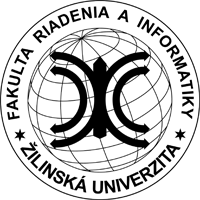
\includegraphics[scale=2,keepaspectratio=true]{./FRI_RGB_SK.png}
 % FRI_RGB_SK.png: 200x200 pixel, 300dpi, 1.69x1.69 cm, bb=0 0 48 48

\textsc{\newline\LARGE Žilinská univerzita v Žiline}\\[0.5cm]

\textsc{\Large Fakulta riadenia a informatiky}\\[0.5cm]

% Title
\HRule \\[0.4cm]
{ \huge \bfseries Analýza diferenčnej rovnice \\[0.4cm] }

\HRule \\[1.5cm]

% Author and supervisor
\begin{minipage}{0.4\textwidth}
\begin{flushleft} \large
\emph{Autori:}\\
Matejko Peter\\
Mudrák Ľuboš\\
Rehák Tomáš\\
Zárecký Martin\\
Boďa Michal\\
Kapusta Peter
\end{flushleft}
\end{minipage}
\begin{minipage}{0.4\textwidth}
\begin{flushright} 
\end{flushright}
\end{minipage}

\vfill

% Bottom of the page
{\large \today}

\end{center}
\end{titlepage}


\newpage

\tableofcontents



\newpage
\section{Zadanie}

V závislosti od hodnôt $ a \text{ a } b $
analyzujte riešenia danej diferenčnej rovnice\linebreak[4]
$x_{n+1}=\left(a+{\frac{b}{n}}\right)\,x_{n}$
kde $ a \text{ a } b $ sú reálne čísla, také, že $ a + b > 0$. Výsledky ilustrujte na jednoduchých príkladoch. 

Budeme skúmať dopady zmeny jednotlivých premenných $a$ a $b$ na riešenia danej diferenčnej rovnice.

\section{Definície}
\subsection{Pojem diferencia}

\begin{defin}
Je daný bod $x_{0}$ a číslo $h > 0$. Nech funkcia $y = f(x)$ je 
definovaná v bodoch $x_{0} \text{ a } x_{0} + h$. \textit{Diferencia funkcie }$f(x)$\textit{ v bode }$x_{0}$
je číslo $f(x_{0} + h) - f(x_{0})$. Značíme
$$\Delta f(x_{0}) = f(x_{0} + h) - f(x_{0})$$
\end{defin}
\subsection{Pojem diferenčná rovnica}
\subsubsection{Typy diferenčných rovníc}

\begin{defin}
(Diferenčné rovnice 1. typu) 
Nech pre všetky $x \in M$ je
definovaná funkcia $f(x, y, \Delta y, \Delta ^{2}y, \ldots, \Delta ^{k}y)$. Rovnica tvaru
$$f(x, y, \Delta y, \Delta ^{2}y, \ldots, \Delta ^{k}y) = 0 \text{ ,}$$
v ktorej neznámou funkciou $y = \varphi(x)$, nazývame diferenčnú rovnicu k-teho 
rádu a 1. typu definovanú v $M$.
\end{defin}

\textbf{\textit{Partikulárnym riešením}} tejto rovnice v $M$ nazveme každú funkciu
$y = \varphi(x)$, ktorá pre všetky $x \in M$ spĺňa danú rovnicu.

\paragraph{}
\textbf{\textit{Všeobecným riešením}} nazývame množinu všetkých partikulárnych
riešení.

\paragraph{}
\begin{defin}
(Diferenčné rovnice 2. typu)
Nech je pre všetky $x \in M$
definovaná funkcia
$$g(x, y_{x}, y_{x+1}, \ldots, y_{x+k})\text{, kde }y_{x+j} = \varphi(x + j) j = 0, 1, 2, \ldots, k\text{.}$$
\end{defin}

Rovnicu tvaru
$$g(x, y_{x}, y_{x+1}, \ldots, y_{x+k}) = 0\text{,}$$
v ktorej neznáma funkcia $y_{x} = \varphi(x)$, nazývaná \textit{diferenčná rovnica 2.typu}
definovaná v $M$. Ak je závislosť $g$ na $y_{x}$ a $y_{x+k}$ nekonštantná hovoríme,
že rovnica \textit{je k-teho rádu}. Riešenie rovnice v $M$ nazývame každú funkciu
$y_{x} = \varphi(x)$, ktorá pre všetky $x \in M$  spĺňa danú rovnicu. K tomu je nutné,
aby definičný obor funkce $\varphi(x)$ obsahoval všetky $x \in M$ a taktiež body
$x + 1, x + 2, \ldots, x + k$.
\newpage
\subsubsection{Rekurentná formula}
Rekurentnú formulu vieme získať z diferenčnej rovnice vyjadrením $(n+k)$-teho člena pomocou $k$ predchádzajúcich členov rovnice.

\paragraph{}
Majme danú diferenčnú rovnicu: $$g(x, y_{x}, y_{x+1}, \ldots, y_{x+k}) = 0\text{.}$$

\begin{enumerate}
	\item Nech definičný obor tejto rovnice sú prirodzené čísla $ n = 1, 2, 3, \ldots a$
		ďalej zaveďme všeobecnejšie označenie pre členy postupnosti: $ y_{n} =  a_{n}$,
		takže rovnicu vieme prepísať ako  $$g(n, a_{n}, a_{n+1}, \ldots, a_{n+k}) = 0\text{.}$$
		Predpokladajme, že túto rovnicu vieme jednoznačne rozriešiť vzhľadom k $ a_{n+k}$ :
		$$a_{n+k} = G(n, a_{n}, a_{n+1}, \ldots, a_{n+k-1})\text{,}$$
		kde $G$ je funkcia, ktorú sme dostali riešením pôvodnej rovnice.\linebreak[4]
		 Dostali sme vlastne všeobecný rekurentný vzorec pre postupnosť $a_{n}$,\linebreak[4] v ktorom je $(n+k)$-ty 				člen vyjadrený pomocou $k$ predchádzajúcich členov 
		$a_{n}, a_{n+1}, \ldots, a_{n+k-1}$ a premennej $n$.
	\item Pozrime sa na riešenie, keď máme vopred dané (ľubovoľné) čísla $ a_{1}, a_{2}, \ldots, a_{k}$.
		Vieme, že po dosadení členov do funkcie $G$ vypočítame jednoznačne člen
		$$a_{k+1} = G(1, a_{1}, a_{2}, \ldots, a_{k};)\text{,}$$ ďalším dosadením vypočítame
		$$a_{k+2} = G(2, a_{2}, a_{3}, \ldots, a_{k+1};)\text{atď.}$$
		Všeobecný $n$-tý člen an dostaneme vypočítaním elementárnej funkcie
		$n$ a daných $k$ prvých čísiel $ a_{1}, a_{2}, \ldots, a_{k}$. Táto funkcia je práve partikulárnym riešením 				diferenčnej rovnice s počiatočnými podmienkami $ a_{1}, a_{2}, \ldots, a_{k}$.	
\end{enumerate}

Touto druhou úvahou sa súčasne znovu potvrdzuje, že všeobecné riešenie rovnice $k$-teho rádu 
$a_{n+k} = G(n, a_{n}, a_{n+1}, \ldots, a_{n+k-1})$ má obsahovať
$k$ všeobecných konštant, ktoré je možno si ľubovoľne zvoliť.

\newpage
\section{Vypracovanie}
\subsection{Triviálne riešenie}
Nech $x_{1}=0$, potom dostávame triviálne riešenie $x_{n+1} = 0$ a teda každý člen postupnosti bude mať hodnotu $0$. Ďalej, v našom vypracovaní, budeme predpokladať, že $ x_{1} > 0 $ a teda sa budeme 
zaoberať závislosťou od hodnôt $ a,b $.

\subsection{Závislosť od hodnôt a, b}
Nech $b=0$,  $x_{1}>0$.\newline
Potom rovnica $x_{n+1}=\left(a+{\frac{b}{n}}\right)\,x_{n}$  nadobudne tvar  $x_{n+1}= a*x_{n}$.
Teda každý ďalší člen postupnosti - $x_{n+1}$ je $a$-násobkom predchádzajúceho člena  $x_{n}$.
Dosadením  $b=0$ teda vzniká z našej rovnice Geometrická postupnosť.
\newpage
\section{Záver}


\begin{thebibliography}{9}
\bibitem{pra}{\em Prágerová, A.:}
               {\bf Diferenční rovnice.}
           Polytechnická knižnice, Praha 1971.
\end{thebibliography}

\end{document}
